\documentclass[letterpaper,12pt]{article}

\usepackage{tabularx} % extra features for tabular environment
\usepackage{amsmath}  % improve math presentation
\usepackage{amssymb}
\usepackage{multirow}
\usepackage{xcolor}
\usepackage{gensymb}
\usepackage{appendix}
\usepackage{verbatim}
\usepackage{bigints}
\usepackage[ruled,vlined]{algorithm2e}
\usepackage{mathtools}
\usepackage{gensymb}
\usepackage{float}
\usepackage{listings}
\usepackage[export]{adjustbox}
\usepackage[super]{nth}
\usepackage{graphicx} % takes care of graphic including machinery
\usepackage[margin=1in,letterpaper]{geometry} % decreases margins
\usepackage{cite} % takes care of citations
\usepackage[final]{hyperref} % adds hyper links inside the generated pdf file

\newcommand*{\tran}{^{\mkern-1.5mu\mathsf{T}}}
\DeclarePairedDelimiter\ceil{\lceil}{\rceil}
\DeclarePairedDelimiter\floor{\lfloor}{\rfloor}
\hypersetup{
    colorlinks=false,       % false: boxed links; true: colored links
    linkcolor=blue,        % color of internal links
    citecolor=blue,        % color of links to bibliography
    filecolor=magenta,     % color of file links
    urlcolor=blue         
}
%++++++++++++++++++++++++++++++++++++++++++++++++++++++++++++++++++++++++++++++++



%++++++++++++++++++++++++++++++++++++++++++++++++++++++++++++++++++++++++++++++++
% Start modifying the labwork number, your team number and the name and METU id
% of your group members.
\newcommand{\reporttitle}{Term Project}
\newcommand{\reportauthor}{ Volkan Aydıngül (Id: 0075359 )\\
                            }
                            % If any teammate does not help to write this report,
                            % you may not write his/her name here.
%++++++++++++++++++++++++++++++++++++++++++++++++++++++++++++++++++++++++++++++++



%++++++++++++++++++++++++++++++++++++++++++++++++++++++++++++++++++++++++++++++++
% DO NOT MODIFY THIS SECTION
\begin{document}
\begin{titlepage}
\newcommand{\HRule}{\rule{0.7\linewidth}{0.5mm}}
\begin{center} % Center remainder of the page
%	LOGO SECTION

\includegraphics[width = 8cm]{figures/koc_logo.png}

%	HEADING SECTIONS
\textsc{\Large PHYS 514 - Computational Physics}\\[1.5cm] 
%	TITLE SECTION
\HRule \\[0.6cm]
{ \huge \bfseries \reporttitle}\\ % Title of your document
\HRule \\[1.5cm]
\end{center}
\vspace{2cm}
%	AUTHOR SECTION
\begin{flushleft} \large
\textit{Author:}\\
\reportauthor% Your name
\end{flushleft}
\vspace{2cm}
\makeatletter
Date: \@date 
\vfill % Fill the rest of the page with whitespace
\makeatother
\end{titlepage}
%++++++++++++++++++++++++++++++++++++++++++++++++++++++++++++++++++++++++++++++++




\tableofcontents
\newpage





%\begin{figure}[H] 
%   \centering \includegraphics[width=\columnwidth]{figures/figure.png}           
%                \caption{Caption}                
%                   \label{fig:label}
%   \end{figure}


\begin{abstract}
    Abstract.
\end{abstract}
\section{Introduction}


\section{Mathematical Background}
\subsection{Newtonian Approach}

\subsubsection{Derivation of \textit{Lane-Emden Equation}}

\paragraph{} In this project, the first task is to derive the \textit{Lane-Emden} equation to be able to have a general expression for the \textit{hydrostatic equilibrium}. In the beginning, it is known that:

\begin{equation}
    \label{eq:dmdr}
    \frac{dm}{dr} = 4\pi r^2\rho
\end{equation}

\begin{equation}
    \label{eq:dpdr}
    \frac{dp}{dr} = -\frac{Gm\rho}{r^2}
\end{equation}

where $m$, $\rho$, and $p$ are functions of $r$. To be able to solve this system of differential equations, the expression for the $\rho$ is required, which is not explicitly given. However, by using the \textit{equation of state (EOS)}, one can easily construct a relation between $p$ and $\rho$, such that:

\begin{equation*}
    p = \frac{k_B}{\mu m_H}T\rho
\end{equation*}

Assuming that isentropic relation holds, one can conclude that:

\begin{equation}
    \label{eq:istro}
    p = K\rho^\gamma=K\rho^{1 + \frac{1}{n}} 
\end{equation}

\paragraph{} To be able to obtain a unified expression, one can inspect the \textit{mass} variable in the \eqref{eq:dmdr}, and \eqref{eq:dpdr}. It is required to calculate the derivative of the \eqref{eq:dpdr} to write \eqref{eq:dpdr} in terms of \eqref{eq:dmdr}. Differentiating \eqref{eq:dpdr} yields:

\begin{equation}
    \label{eq:d2pdr2-1}
    \frac{d^2p}{dr^2} = \frac{2Gm\rho}{r^3} + \frac{-G\rho}{r^2}\frac{dm}{dr} + \frac{-Gm}{r^2}\frac{d\rho}{dr}
\end{equation}

\paragraph{} Before further processing on the \eqref{eq:d2pdr2-1}, the some terms must be revised, that is, \eqref{eq:d2pdr2-1} can be rewritten in the following form:

\begin{equation}
    \label{eq:d2pdr2-2}
    \frac{d^2p}{dr^2} = \frac{2}{r}\left(-\frac{dp}{dr}\right) + \frac{d\rho}{dr}\left(\frac{1}{\rho}\frac{dp}{dr}\right) + 4\pi G \rho^2
\end{equation}

\paragraph{}Multiplying \eqref{eq:d2pdr2-2} with $\frac{r^2}{\rho}$ and rearranging the terms yields:

\begin{equation}
    \label{eq:totder-1}
    \frac{r^2}{\rho}\frac{d^2p}{dr^2} + 2r\left(\frac{1}{\rho}\frac{dp}{dr}\right) - r^2\frac{d\rho}{dr}\left(\frac{1}{\rho^2}\frac{dp}{dr}\right) = 4\pi G r^2 \rho
\end{equation}

\paragraph{}Observing \eqref{eq:totder-1}, one can easily realize that the left hand side is nothing but the total derivative of the term $\frac{r^2}{\rho}\frac{dp}{dr}$. Hence, in conclusion, the \eqref{eq:d2pdr2-1}, can be written as the following:

\begin{equation}
    \label{eq:totder-2}
    \frac{d}{dr}\left(\frac{r^2}{\rho}\frac{dp}{dr}\right) = 4\pi G r^2 \rho
\end{equation}

\paragraph{} From now on, the finite amount of transformation should be applied on the $\rho$ and $r$. Firstly, assume that the following relations hold:

\begin{equation*}
    %\theta = \rho^{\frac{1}{n}} \rightarrow \rho = \theta^n
    \rho = \rho_c \theta^n
\end{equation*}

Therefore, 

\begin{equation}
    \label{eq:dp}
    p = K \rho_c^{1+\frac{1}{n}} \theta^{n+1} \rightarrow dp = K \rho_c^{1+\frac{1}{n}} \left(n+1\right)\theta^n d\theta
\end{equation}

\paragraph{} Applying \eqref{eq:dp} to \eqref{eq:totder-2}, one can write:

\begin{equation}
    \frac{d}{dr}\left(\frac{r^2}{\rho_c \theta^n} K \rho_c^{1+\frac{1}{n}} \left(n+1\right)\theta^n \frac{d\theta}{dr}\right) = 4\pi G r^2 \rho_c \theta^n \rightarrow \frac{1}{r^2}\frac{d}{dr}\left(r^2 \frac{K \rho_c^{\frac{1}{n}-1} \left(n+1\right)}{4 \pi G} \frac{d\theta}{dr}\right) + \theta^n = 0
\end{equation}

\paragraph{} Followingly, another transformation that should be applied might be:

\begin{equation}
    \label{eq:alpha}
    \alpha^2 = \frac{K \rho_c^{\frac{1}{n}-1} \left(n+1\right)}{4 \pi G} \rightarrow r = \alpha \xi
\end{equation}

\paragraph{} Then, \eqref{eq:totder-2} can be written as:

\begin{equation*}
    \left(\frac{1}{\alpha^2}\frac{1}{\xi^2}\right)\frac{1}{\alpha}\frac{d}{d\xi}\left(\alpha^2\xi^2\alpha^2\frac{1}{\alpha}\frac{d\theta}{d\xi}\right) + \theta^n = 0
\end{equation*}

\begin{equation}
    \label{eq:final}
   \frac{1}{\xi^2}\frac{d}{d\xi}\left(\xi^2\frac{d\theta}{d\xi}\right) + \theta^n = 0
\end{equation}

\paragraph{} The approximate solution of the \eqref{eq:final} via \textit{Wolfram Mathematica} reads:

\begin{equation*}  
      \theta(\xi) =  1-\frac{\xi ^2}{6}+\frac{n \xi ^4}{120}+\frac{n (5-8 n) \xi ^6}{15120}+\dots
\end{equation*}

\paragraph{} For $n = 1$, solution can be written as:

\begin{equation*}
    \theta(\xi) =  \frac{\sin (\xi )}{\xi }
\end{equation*}

\subsubsection{Calculation of Total Mass}

\paragraph{} To be able to calculate the mass of the star for a given radius, one can easily make use of the \eqref{eq:dmdr}, that is, integration of the \eqref{eq:dmdr} for a certain radius interval yields the mass of the subject star. That being said, the following relation can be observed:

\begin{equation*}
   M =  \int_0^R {4\pi r^2 \rho(r)}dr
\end{equation*}

After the change of variables,

\begin{equation*}
    M = \int_0^{\xi_*} {4 \pi \alpha^2 \xi^2 \rho_c \theta^n (\xi)} \alpha d\xi
\end{equation*}
where ${\xi_*} = \frac{R}{\alpha}$
\begin{equation*}
    M =4 \pi \rho_c \alpha^3 \int_0^{\xi_*} {\xi^2 \theta^n (\xi)} d\xi
\end{equation*}

\paragraph{} By using the relation in \eqref{eq:final}, one can deduce that:

\begin{equation*}
    M =4 \pi \rho_c \alpha^3 \int_0^{\xi_*} -{\xi^2 \frac{1}{\xi^2}\frac{d}{d\xi}\left(\xi^2\frac{d\theta}{d\xi}\right) } d\xi
\end{equation*}

\begin{equation*}
    M = 4 \pi \rho_c \alpha^3 {\xi_*}^2 \theta' = 4 \pi \rho_c \alpha^3 {\xi_*}^3 \frac{-\theta'}{{\xi_*}}
\end{equation*}
\paragraph{} Finally, the total mass can be read as:
\begin{equation}
    \label{eq:mass}
\boxed{ M = 4 \pi \rho_c R^3 \frac{-\theta'}{{\xi_*}}}
\end{equation}


\subsubsection{Relation Between Mass and Radius}

\paragraph{} For a group of stars sharing same polytopic EOS, one can write a common relation between mass and radius. The first thing that should be implemented is previous version of the \eqref{eq:mass}:
\begin{equation*}
    M = 4 \pi \rho_c \alpha^3 {\xi_*}^2 \theta' = 4 \pi \rho_c \alpha^3 {\xi_*}^3 \frac{-\theta'}{{\xi_*}}
\end{equation*}

Replacing $\alpha$ with \eqref{eq:alpha}:

\begin{equation*}
    M = 4 \pi \left[\frac{K \rho_c^{\frac{1}{n}-1}\left(n+1\right)}{4 \pi G}\right]^{\frac{3}{2}} \rho_c \xi_*^2 \left[-\theta'(\xi_*)\right]
\end{equation*}

Rearranging the terms:

\begin{equation}
    \label{eq:mass2}
    M = 4 \pi \left[\frac{K\left(n+1\right)}{4 \pi G}\right]^{\frac{3}{2}} \rho_c^{\frac{3-n}{2n}} \xi_*^2 \left[-\theta'(\xi_*)\right]
\end{equation}

\paragraph{} At the same time, one should consider the \textit{radius} equation, which reads:

\begin{equation}
    \label{eq:radius}
    R = \alpha \xi_* = \left[\frac{K \rho_c^{\frac{1}{n}-1}\left(n+1\right)}{4 \pi G}\right]^{\frac{1}{2}}\xi_* = \left[\frac{K \left(n+1\right)}{4 \pi G}\right]^{\frac{1}{2}} \rho_c^{\frac{1-n}{2n}} \xi_*
\end{equation}

\paragraph{} Now, to be able to construct a relation between mass and radius assuming that the group of stars share same polytopic properties, the $\rho_c$ term should be eliminated from the equation. Therefore, the second process that should be implemented is to find an expression for the $\rho_c$, from which \eqref{eq:mass2} :

\begin{equation}
    \label{eq:rho_c}
    \rho_c = \left[\frac{M}{4 \pi} \left[\frac{4 \pi G}{K \left(n+1\right)}\right]^{\frac{3}{2}}  \frac{1}{\xi_*^2\left(-\theta'(\xi_*)\right)}\right]^{\frac{2n}{3-n}}
\end{equation}

Plugging \eqref{eq:rho_c} into \eqref{eq:radius}:

\begin{equation*}
    R = \left[\frac{K \left(n+1\right)}{4 \pi G}\right]^{\frac{1}{2}} \left[\frac{M}{4 \pi} \left[\frac{4 \pi G}{K \left(n+1\right)}\right]^{\frac{3}{2}}  \frac{1}{\xi_*^2\left(-\theta'(\xi_*)\right)}\right]^{\frac{1-n}{3-n}} \xi_* 
\end{equation*}

\begin{equation*}
    R =  \left[\frac{K \left(n+1\right)}{4 \pi G}\right]^{\frac{1}{2}} \left[\frac{1}{4 \pi} \left[\frac{4 \pi G}{K \left(n+1\right)}\right]^{\frac{3}{2}}  \frac{1}{\xi_*^2\left(-\theta'(\xi_*)\right)}\right]^{\frac{1-n}{3-n}} \xi_* M^{\frac{1-n}{3-n}} 
\end{equation*}

which asserts that:

\begin{equation*}
    M \propto R^{\frac{3-n}{1-n}}
\end{equation*}

\paragraph{} Finally, the constant of proportionality can be written as:

\begin{equation}
    \label{eq:mass-radius-prop}
    M = C(K, n, \xi_*, \theta') R^{\frac{3-n}{1-n}} 
\end{equation}
where 

\begin{equation}
    \label{eq:const-prop}
  \boxed{  C(K, n, \xi_*, \theta') = \frac{ \left[\frac{K \left(n+1\right)}{4 \pi G}\right]^{\frac{n-3}{2 - 2n}} }{\frac{1}{4 \pi} \left[\frac{4 \pi G}{K \left(n+1\right)}\right]^{\frac{3}{2}}  \frac{1}{\xi_*^2\left(-\theta'(\xi_*)\right)}} \xi_*^{\frac{n-3}{1-n}} }
\end{equation}

\subsubsection{Special Case for White Dwarfs}

\paragraph{} White dwarfs are the final stages of the low-mass stars where the pressure-density relation does not governed by the polytopic relation. In the case of white dwarfs, the main mechanism that governs the star is the quantum mechanical effect called \textit{electron degeneracy}. In the case of \textit{electron degeneracy}, the pressure-density relation can be written as:

\begin{equation}
    \label{eq:P-rho-low}
    P = C \left[x \left(2x^2-3\right)\left(x^2+1\right)^{\frac{1}{2}}+3\sinh^{-1}{x}\right]
\end{equation}

where $x = \left(\frac{\rho}{D}\right)^{\frac{1}{q}}$

\paragraph{} Finally, if the $x<<1$ , then the \eqref{eq:P-rho-low} can be reduced to via \textit{series expansion}:

\begin{equation*}
    P = \frac{8}{5} \left(\frac{\rho}{D}\right)^{\frac{5}{q}}
\end{equation*}

\paragraph{} This form can be easily transformed into the \textit{polytropic} assemble, as demonstrated in the following expression:
\begin{equation}
    \label{eq:P-rho-low-reduced}
    P = K_* \rho^{1 + \frac{1}{n_*}}
\end{equation}

where $K_* = \frac{8C}{5D^{\frac{5}{q}}}$ and $n_* = \frac{q}{5-q}$

\subsection{Relativistic Approach}

\paragraph{} When the mass of a white dwarf exceeds the special limit called \textit{Chandrasekar limit}, it is tended to explode. However, even after the explosion, some of them might have a core that is heavier than the \textit{Chandrasekar limit}. In this case, if the mass is not too large, a special type of star called \textit{Neutron star (NS)} is formed. For a NS, the \textit{Newtonian} approach does not further hold, hence, the relativistic approach should be considered.

\subsubsection{Tolman-Oppenheimer-Volkoff (TOV) Equation}
\label{sec:tov}
\paragraph{} When the general relativistic effects are considered, the \eqref{eq:dmdr} and \eqref{eq:dpdr} is being transformed into the following structure:

\begin{equation}
\begin{aligned}
    \label{eq:tov}
    m' &= 4 \pi r^2 \rho \\
    \nu' &= 2 \frac{m + 4 \pi r^3 p}{r \left(r - 2m\right)} \\
    p' &= -\frac{m + 4 \pi r^3 p}{r \left(r - 2m\right)} \left(\rho + p\right) = -\frac{1}{2}\left(\rho + p\right)\nu'
\end{aligned}
\end{equation}

where $m$, $\rho$ and $p$ represent the mass, density and pressure, respectively, and, $\nu$ represents \textit{time dilation}. As usual, to be able to solve \eqref{eq:tov}, one should obtain a relation between density and pressure. Although, there is not any well-defined equation of state for relativistic case, the polytropic EOS with polytropic index of $1$ is a proper approximation. That is:

\begin{equation*}
    p = K_{NS} \rho ^ 2
\end{equation*}

\paragraph{} Finally, \eqref{eq:tov} can be solved via integrating from the following initial conditions:

\begin{equation*}
    \begin{aligned}
        m(0) &= 0\\
        \nu(0) &= 0\\
        p(0) &= p_c
    \end{aligned}
\end{equation*}

where $p_c$ denotes the central pressure.

\subsubsection{Fractional Binding Energy}

\paragraph{} Due to the relativistic effects, the calculated mass via using the \eqref{eq:tov} does not represent the sum of the rest mass, since there is also negative contribution from the binding energy. However, the rest mass can be found via adding the following ODE to the set of \eqref{eq:tov}:

\begin{equation*}
    m_p' = 4 \pi \left(1 - \frac{2m}{r}\right)^{-\frac{1}{2}}r^2\rho
\end{equation*}

where $m_p$ represents the baryonic mass. Finally, the \textit{fractional binding energy} can be calculated via using the following formulation:

\begin{equation*}
    \Delta = \frac{M_p - M}{M}
\end{equation*}

\subsubsection{Outside the Star}
\paragraph{} It can be easily acknowledged that there is not any mass and pressure outside the star, which means $m(r>R) = M$ and $p(r>R) = 0$. Therefore, the only equation to be solved is the reduced form of the time dilation, that is for $r>R$:

\begin{equation*}
    \nu' = \frac{2M}{r\left(r - 2M\right)}
\end{equation*}

\paragraph{} Using \textit{Wolfram Mathematica}, it can be shown that:

\begin{equation}
    \label{eq:v1}
    \nu(r) = -\ln(r) + \ln(r -2M) + C
\end{equation}

\paragraph{} Also, it is known that the addition of a constant does not change the solution. Therefore, firstly, the $\nu(R)$ should be calculated, which reads:

\begin{equation}
    \label{eq:v2}
    \nu(R) = -\ln(R) + \ln(R -2M) + C
\end{equation}

\paragraph{}Finally, the substraction of \eqref{eq:v2} from \eqref{eq:v1} and the rearrangement of the terms yields:

\begin{equation*}
    \nu(r>R) = \ln(1-\frac{2M}{r}) - \ln(1-\frac{2M}{R})+\nu(R) 
\end{equation*}



\section{Experiments}
\subsection{Interpreting the Raw Data}
\paragraph{} First of all, it should be acknowledged that the interpreting of the raw data is a very hard practice. In this section, the subject data will be briefly reviewed and the numerical approachs that is used to process the data will be explained.

\subsubsection{White Dwarf Data}

\paragraph{} The white dwarf data consists of the mass and radius information of the 378 stars. The mass and radius informations are given in the form of \textit{solar mass} and $\mathit{log(g)}$, respectively. To be able to work in SI units, some conversion must be done. The most trivial conversion is possibly the one that involves the solar mass. The solar mass can be converted to the \textit{kilogram} counterpart via using the following formulation:

\begin{equation*}
    1 M_\odot = 1.98847 \times 10^{30} \; kg
\end{equation*}

\paragraph{} Then, to be able to find the radius in \textit{meters}, one can make use of the \textit{Newton' Law of Gravitation}, which reads:

\begin{equation*}
    g = 10 ^ {L} S
\end{equation*}

where $L$ is the radius in $\mathit{log(g)}$, and $S = 0.01$ is the scaler factor that convert the $g$ value in CGS to SI. It is known that:

\begin{equation*}
    g = \frac{GM}{R^2}
\end{equation*}

Then, the radius $R$ in \textit{meters}, can be written as:

\begin{equation*}
    R = \sqrt{\frac{GM}{g}}
\end{equation*}

\subsection{Calculation of Mass and Radius in Newtonian Approach}
\paragraph{} Tha mass and radius can simply be calculated via the integration of the \eqref{eq:final}  from center to the outer surface, that is until $\theta(\xi_*) = 0$. Based on the condition, also, the \eqref{eq:dmdr} and \eqref{eq:dpdr} can be used to calculate mass and radius relation.

\subsection{Estimation of $K_*$ and $q$ in Newtonian Approach}
\label{sec:Kq_fit}
\paragraph{} The first thing that should be done is to make use of the \eqref{eq:mass-radius-prop} and \eqref{eq:P-rho-low-reduced}, since they include the variables that are inherent in \textit{White Dwarf} data and the simplification that makes the numerical processes easier. Note that the \eqref{eq:P-rho-low-reduced} is only valid for $x<<1$, which forces to limit the data that will be used in the numerical process. For the time being, accept that the data that will be used has the following property:

\begin{equation*}
    M \leqslant M_{threshold}
\end{equation*}

\paragraph{} The effect of the different variations of the $M_{threshold}$ is discussed in the Section \ref{sec:resdis}. To be able to find $K_*$ and $q$, one can construct a \textit{curve-fitting} pipeline, which takes into account \eqref{eq:mass-radius-prop} and \eqref{eq:P-rho-low-reduced}, since the \eqref{eq:P-rho-low-reduced} is the direct implication of the fact that \textit{Lane Emden} equation can be considered valid. In the beginning, it can be assumed that the mass and radius can be related via the following imaginary function:

\begin{equation}
    \label{eq:Kq_fit}
    M = f(R, K_*, q)
\end{equation}

\paragraph{} The \eqref{eq:Kq_fit} can be expanded in two different ways, which ultimately determines the fitting pipeline.

\subsubsection{Alternative 1}
\label{sec:Kq_fit_a1}

\paragraph{} The first alternative can be the fact that mass can be related to the radius in an exponential form with a scaling factor, that is being inspired by the \eqref{eq:mass-radius-prop}:

\begin{equation*}
    M = A R^{\frac{3-n}{1-n}}
\end{equation*}

\paragraph{} where the $n = \frac{q}{q-5}$. In this form, one can easily implement a \textit{non-linear curve-fitting} procedure to find constants $A$ and $q$. Once the $A$ is found, a little bit of algebraic manipulation is required to find the $K_*$. From \eqref{eq:const-prop}, it is known that:


\begin{equation*}
   A =\frac{ \left[\frac{K_* \left(n+1\right)}{4 \pi G}\right]^{\frac{n-3}{2 - 2n}} }{\frac{1}{4 \pi} \left[\frac{4 \pi G}{K_* \left(n+1\right)}\right]^{\frac{3}{2}}  \frac{1}{\xi_*^2\left(-\theta'(\xi_*)\right)}} \xi_*^{\frac{n-3}{1-n}}
\end{equation*}

\paragraph{}Assume that:

\begin{equation*}
    B = \left[\frac{n+1}{4\pi G}\right]^{\frac{-2n}{2-2n}} \xi_*^{\frac{-n-1}{1-n}} 4 \pi \left( -\theta'(\xi_*) \right)
\end{equation*}

\paragraph{} Then, after some algebraic manipulations, one can obtain:

\begin{equation*}
    K_* = \left(\frac{A}{B}\right) ^ {\frac{n-1}{n}}
\end{equation*}

\paragraph{} Here, note that the solution of the IVP (\textit{Lane Emden equation}) is required to obtain $\xi_*$ and $\theta'(\xi_*)$, where $\xi_*$ refers to the $\xi$ value when $r = R$. All in all, this alternative is very cheap in terms of the required operations in one step, and it is very simple in terms of the mathematical equation that is imposed on the \textit{non-linear curve-fitting} subroutine.

\subsubsection{Alternative 2}
\label{sec:Kq_fit_a2}

\paragraph{} The second alternative is to use the \eqref{eq:mass-radius-prop} directly, which reads:

\begin{equation}
    \label{eq:M-R-long}
    M = \left[\frac{ \left[\frac{K_* \left(n+1\right)}{4 \pi G}\right]^{\frac{n-3}{2 - 2n}} }{\frac{1}{4 \pi} \left[\frac{4 \pi G}{K_* \left(n+1\right)}\right]^{\frac{3}{2}}  \frac{1}{\xi_*^2\left(-\theta'(\xi_*)\right)}} \xi_*^{\frac{n-3}{1-n}} \right] R^{\frac{3-n}{1-n}}
\end{equation}

\paragraph{} To \eqref{eq:M-R-long}, one one can easily implement a \textit{non-linear curve-fitting} procedure to find constants $K_*$ and $q$. However, the negative side of this scheme is that it requires a solution of an IVP (\textit{Lane Emden equation}) in each step, which can be computationaly very demanding.

\subsubsection{Further Improvement}
\label{sec:Kq_fit_f}

\paragraph{} Theoretically, it is known that $q$ should be an integer. However, during \textit{non-linear curve-fitting process}, it is very hard to impose that constraint. Therefore, one further improvement might be, firstly, the calculation of the $K_*$ and $q$, and then, the second calculation for the only $K_*$ by fixing $q$ to the nearest integer.  


\subsection{Estimation of $C$ and $D$ in Newtonian Approach}
\label{sec:D_fit}
\paragraph{} From \eqref{eq:P-rho-low-reduced}, it is known that:

\begin{equation*}
    C = \frac{5}{8}K_* D^{\frac{5}{q}}
\end{equation*}

\paragraph{} It means that if one is able to make accurate estimation of the $D$, the $C$ can be immediately found, since the $K_*$ is known beforehand. However, at this point, it is very important to approximate D in a most efficient way. 

\subsubsection{Alternative 1}
\label{sec:D_fit_a1}
\paragraph{} To estimate the $D$, the following methodology will be traced. Firstly, one should solve the \eqref{eq:dmdr}, and \eqref{eq:dpdr} in conjunction to be able to obtain the mass and radius information for a given $\rho_c$ value. The reason for the usage of the \eqref{eq:dmdr}, and \eqref{eq:dpdr} as opposed to the \textit{Lane Emden equation} is the fact that \textit{Lane Emden equation} is not valid anymore for white dwarfs. However, as can be seen in \eqref{eq:dpdr}, the pressure equation should be converted to the density equation via using the \eqref{eq:P-rho-low}, such that:

\begin{equation*}
    \frac{dp}{dr} = \frac{dp}{dx} \frac{dx}{d \rho} \frac{d \rho}{dr} 
\end{equation*}

\begin{equation*}
    \frac{d \rho}{dr}  = \frac{ \frac{dp}{dr}}{ \frac{dp}{dx} \frac{dx}{d \rho} }
\end{equation*}

where 

\begin{equation*}
    x = \left(\frac{\rho}{D}\right)^{\frac{1}{q}}
\end{equation*}

\begin{equation*}
    \frac{dp}{dx} =  \left(\left(2  x ^ 2 - 3\right)  (x ^ 2 + 1) ^ {\frac{1}{2}}\right) + \left(4x^2  \left(x ^ 2 + 1\right) ^ {\frac{1}{2}}\right) + \left(x^2 (2  x ^ 2 - 3) \left(x ^ 2 + 1\right) ^ {\frac{1}{2}}\right) + \frac{3}{\sqrt{x ^ 2 + 1}}
\end{equation*}

\begin{equation*}
    \frac{dx}{d \rho} = D^{\frac{-1}{q}} \frac{\rho^{\frac{1}{q} - 1}}{q}
\end{equation*}

\paragraph{} Having that mass and appropriate density equation, one can integrate them via using the following initial conditions:

 \begin{equation*}
     m(0) = 0
 \end{equation*}

 \begin{equation*}
     \rho(0) = \rho_c
 \end{equation*}

 until the $\rho(R) = 0$. Hence, at that particular point, the mass reads $m(R) = M$

 \paragraph{} Secondly, the enough number of $\rho_c$ point should be sampled to construct a representative $M-R$ solution. Once the representative $M-R$ solution is obtained, one can implement a \textit{spline interpolation} on that data and try to approximate to the original $M-R$ data. Finally, with iterating the initial guess of $D$ and trying to minimize the error between representative $M-R$ spline and original $M-R$ data, the final solution for $D$ can be obtained.

 \subsubsection{Alternative 2}
 \label{sec:D_fit_a2}

 \paragraph{} The other alternative might be the usage of the \eqref{eq:P-rho-low-reduced} rather than the usage of the \eqref{eq:P-rho-low}. In this case, the only altering relation is the following:

 \begin{equation*}
    \frac{dp}{dx} = 8Cx^4
 \end{equation*}

 The rest can be implemented in the same way, as is done in Section \ref{sec:D_fit_a1}.


\subsection{Calculation of Mass and Radius in Relativistic Approach}
\paragraph{} Tha mass and radius can simply be calculated via the integration of the \eqref{eq:tov} from center to the outer surface, that is until $p(R) = 0$. Moreover, all other calculations can be implemented on the calculated mass and radius values.
\section{Results and Discussion}
\subsection{Experimental Results Based on the Newtonian Approach}
% TODO: Talk about the difference between fixed q and unfixed q.

\label{sec:resdis}

\paragraph{} From Figure \ref{fig:12} to Figure \ref{fig:11_12}, all figures include side-by-side graphics which represents the whole dataset and the portion of the dataset which satisfies the below relation:

\begin{equation*}
    M \leq M_{threshold}
\end{equation*}

where $M_{threshold}$ is determined as $M_{threshold} = 0.34 \; M_\odot$.

\paragraph{} Moreover, from Figure \ref{fig:12} to Figure \ref{fig:11_12}, the following methods, there are different annotations for the usage of the different methods. To begin with, \textit{Curve Fit for K and q} represents the initial curve-fitting procedure that estimates the $K$ and $q$ concurrently, which is also reflected in numerous alternatives in Section \ref{sec:Kq_fit}. Secondly, \textit{Curve Fit for only K} represents the further improvement that is mentioned in Section \ref{sec:Kq_fit}. Finally, \textit{Curve Fit for Only D} represents the processes took place after the finding of the $K$ and $q$, which is also discussed in Section \ref{sec:D_fit}.


\begin{figure}[H]
\begin{minipage}{.5\textwidth}
\centerline{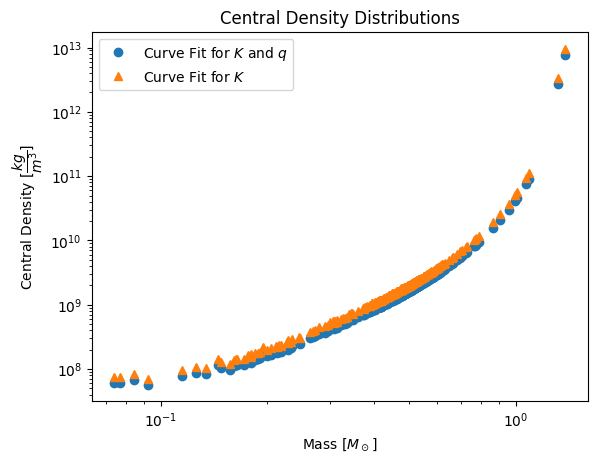
\includegraphics[width=\linewidth]{figures/1_n_ll_rho_m.png}}
%\caption{}
%\label{fig:1_n_ll_rho_m}
\end{minipage}
\begin{minipage}{.5\textwidth}
\centerline{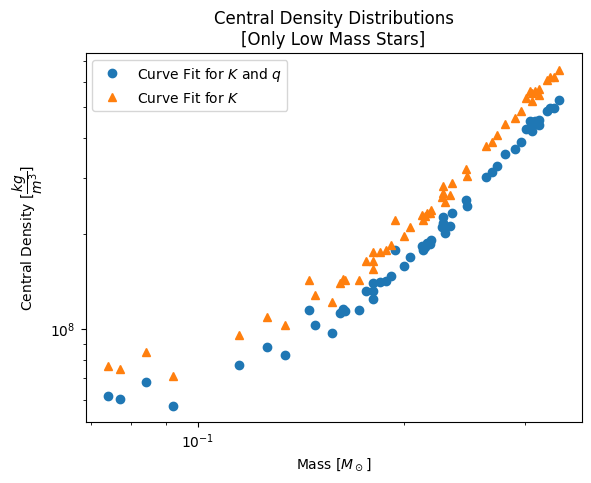
\includegraphics[width=\linewidth]{figures/2_n_ll_rho_m_.png}}
%\caption{}
%\label{fig:2_n_ll_rho_m_}
\end{minipage}
\caption{Central Density Distribution as a \textit{Log-log} plot}
\label{fig:12}
\end{figure}

\paragraph{} In Figure \ref{fig:12} and Figure \ref{fig:34}, the central density distribution that is estimated based on the methods discussed in Section \ref{sec:Kq_fit_a1} and Section \ref{sec:Kq_fit_f} can be visualized. Having observed them, the first comment should be the fact that the further improvement actually does not result in a distinct advancement on the results. However, it should be noted that the main reason behind this fact is the effect of the selected low mass region, which will be discussed in Table \ref{tab:Kq}.

\begin{figure}[H]
\begin{minipage}{.5\textwidth}
\centerline{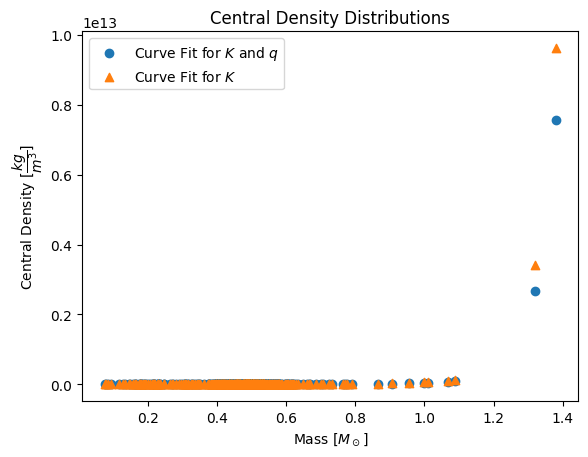
\includegraphics[width=\linewidth]{figures/3_n_s_rho_m.png}}
%\caption{}
%\label{fig:1_n_ll_rho_m}
\end{minipage}
\begin{minipage}{.5\textwidth}
\centerline{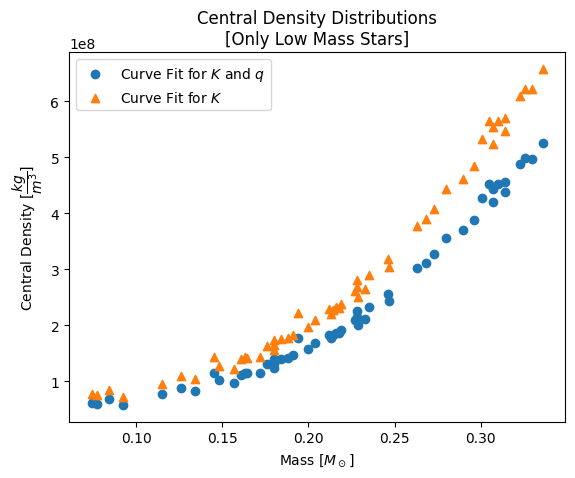
\includegraphics[width=\linewidth]{figures/4_n_s_rho_m_.png}}
%\caption{}
%\label{fig:2_n_ll_rho_m_}
\end{minipage}
\caption{Central Density Distribution as a \textit{Scatter} plot}
\label{fig:34}
\end{figure}



\begin{figure}[H]
\begin{minipage}{.5\textwidth}
\centerline{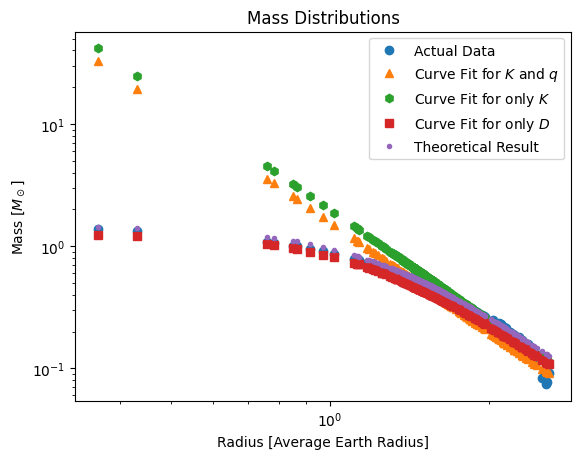
\includegraphics[width=\linewidth]{figures/7_n_ll_ms_r.png}}
%\caption{}
%\label{fig:1_n_ll_rho_m}
\end{minipage}
\begin{minipage}{.5\textwidth}
\centerline{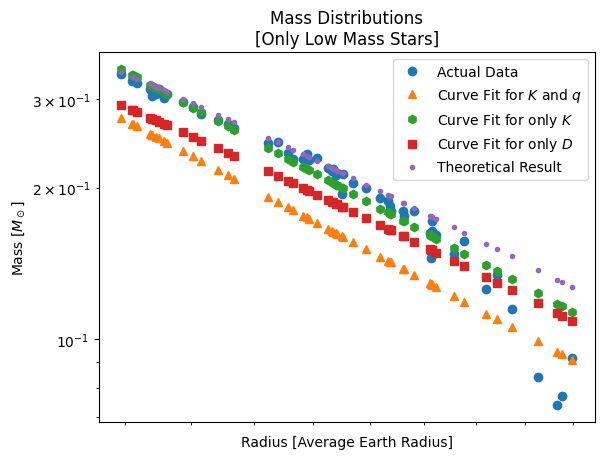
\includegraphics[width=\linewidth]{figures/8_n_ll_ms_r_.png}}
%\caption{}
%\label{fig:2_n_ll_rho_m_}
\end{minipage}
\caption{Mass Distribution as a \textit{Log-log} plot}
\label{fig:78}
\end{figure}


\paragraph{} In Figure \ref{fig:78} and Figure \ref{fig:11_12}, the mass distribution as a function of radius can be observed. In addition to the usage of the methods discussed in Section \ref{sec:Kq_fit_a1} and Section \ref{sec:Kq_fit_f}, to estimate $D$, the method discussed in Section \ref{sec:D_fit_a1} is used. Having observed Figure \ref{fig:78} and Figure \ref{fig:11_12}, one can immediately deduce that the fitting processes applied to find $K$ and $q$ is very succesful to approximate actual data. However, when the broader perpective is considered, it can be observed that the further fitting process on the $D$ provides a better overall accuracy on the actual data. One reason for this fact might be the lack of information during the processes that considers only the $K$ and $q$. Also, from Figure \ref{fig:78}, it can be easily detected that there is a certain boundary that limits the mass, which is actually called \textit{Chandrasekhar limit}.


\begin{figure}[H]
\begin{minipage}{.5\textwidth}
\centerline{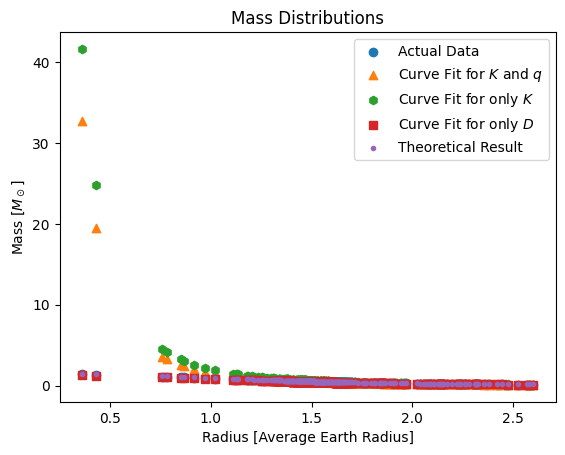
\includegraphics[width=\linewidth]{figures/11_n_s_ms_r.png}}
%\caption{}
%\label{fig:1_n_ll_rho_m}
\end{minipage}
\begin{minipage}{.5\textwidth}
\centerline{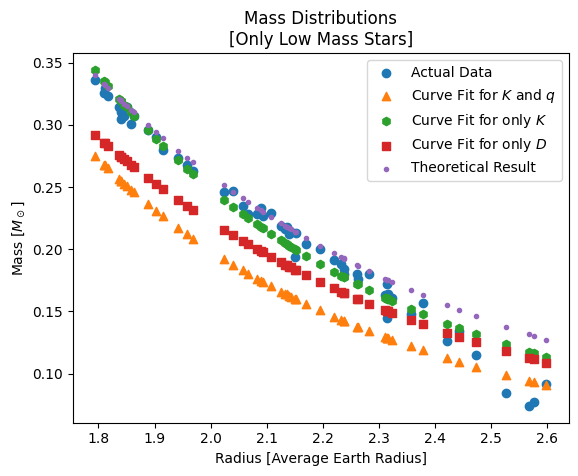
\includegraphics[width=\linewidth]{figures/12_n_s_ms_r_.png}}
%\caption{}
%\label{fig:2_n_ll_rho_m_}
\end{minipage}
\caption{Mass Distribution as a \textit{Scatter} plot}
\label{fig:11_12}
\end{figure}


\begin{table}[H]
\centering
\resizebox{\textwidth}{!}{%
\begin{tabular}{|c|c|c|c|c|}
\hline
\textbf{} & \multicolumn{2}{c|}{\textbf{When K and q are concurrently fitted}} & \multicolumn{2}{c|}{\textbf{When K is fitted while q is fixed}} \\ \hline
\textbf{}                      & \textbf{K} & \textbf{q} & \textbf{K} & \textbf{q} \\ \hline
{$\mathbf{M \leq 0.34 M_\odot}$} & 2677748.44 & 3.0011     & 2850931.98 & 3.0        \\ \hline
{$\mathbf{M \leq 0.50 M_\odot}$} & 131902.29  & 3.0634     & 2725562.65 & 3.0        \\ \hline
\end{tabular}%
}
\caption{Estimation of the $K$ and $q$ under different \textit{low mass} region selections}
\label{tab:Kq}
\end{table}

\paragraph{} One further inspection on the results might be made on the effect of the selection of the \textit{low mass} region. Observing Table \ref{tab:Kq}, one can easily deduce that the selection of the \textit{low mass} region has a great impact on the $K$ and $q$ estimation when they are estimated concurrently. However, it should be also observed that the effect of the \textit{low mass} region selection on $K$ when q is fixed is relatively minimal when it is compared to the previous case. Rougly speaking, one reason for that might be the fact that when the $q$ is not properly constrained, it is not possible to impose the physical interpretation of the \textit{low mass} white dwarf condition on the fitting procedure. In that case, the more proper incorporation of the \textit{low mass} white dwarf condition is being provided by sampling of the mass and radius data. That is, if the all data accurately represents the cluster of \textit{low mass} white dwarfs, it is not required to match all constants to their theoretical counterparts. However, if the constraint on the $q$ is properly imposed on the procedure (i.e. fixing to nearest \textit{integer}), there is not any need to keep the sample so tight. All in all, that is why the estimated $K$ values in the fixed $q$ case are similar while the estimated $K$ values in the unfixed $q$ case are tended to differ.

\paragraph{} Also, the results of the all estimations can be observed in Table \ref{tab:all_param}.

% Please add the following required packages to your document preamble:
% \usepackage{graphicx}
\begin{table}[H]
    \centering
    \resizebox{\textwidth}{!}{%
    \begin{tabular}{|c|c|c|c|c|c|c|}
    \hline
     & \multicolumn{2}{c|}{\textbf{When K and q are concurrently fitted}} & \multicolumn{2}{c|}{\textbf{When K is fitted while q is fixed}} & \textbf{} & \textbf{} \\ \hline
                                   & \textbf{K}       & \textbf{q}     & \textbf{K}      & \textbf{q}    & \textbf{D}          & \textbf{C}             \\ \hline
    $\mathbf{M \leq 0.34 M_\odot}$ & $2677748.44$     & $3.0011$       & $2850931.98$    & $3.0$         & $2.003 \times 10^9$ & $5.674 \times 10^{21}$ \\ \hline
                                   & \multicolumn{2}{c|}{\textbf{K}}   & \multicolumn{2}{c|}{\textbf{q}} & \textbf{D}          & \textbf{C}             \\ \hline
    \textbf{Theoretical}           & \multicolumn{2}{c|}{$3161128.62$} & \multicolumn{2}{c|}{$3.0$}      & $1.947 \times 10^9$ & $6.002 \times 10^{21}$ \\ \hline
    \end{tabular}%
    }
    \caption{Overall Estimated Parameter Set}
    \label{tab:all_param}
    \end{table}

\paragraph{} Finally, the \textit{Chandrasekhar limit} can be observed more clearly in Figure \ref{fig:chandrasekhar}, which corresponds to approximately $M_{ch} \approx 1.5 M_\odot$

\begin{figure}[H] 
   \centering 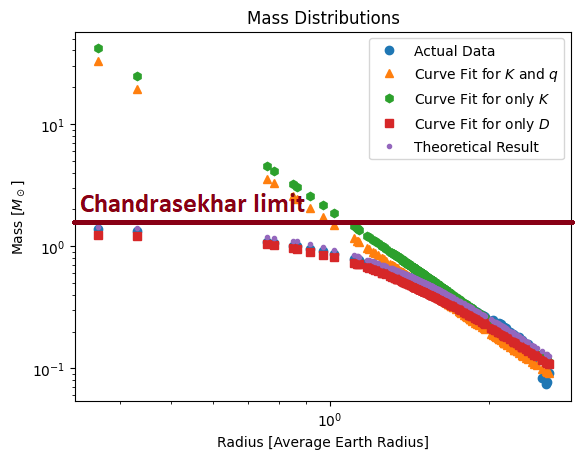
\includegraphics[width=0.7\columnwidth]{figures/7_n_ll_ms_r_chandrasekhar.png}           
                \caption{Visualization of the Chandrasekhar Limit}                
                   \label{fig:chandrasekhar}
   \end{figure}



\begin{comment}
\begin{figure}[H]
\begin{minipage}{.5\textwidth}
\centerline{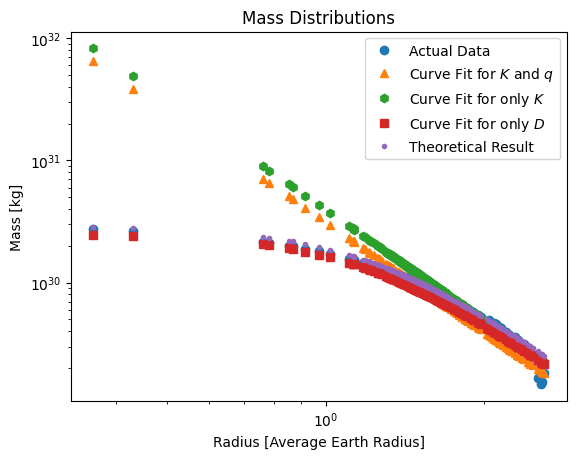
\includegraphics[width=\linewidth]{figures/5_n_ll_m_r.png}}
%\caption{}
%\label{fig:1_n_ll_rho_m}
\end{minipage}
\begin{minipage}{.5\textwidth}
\centerline{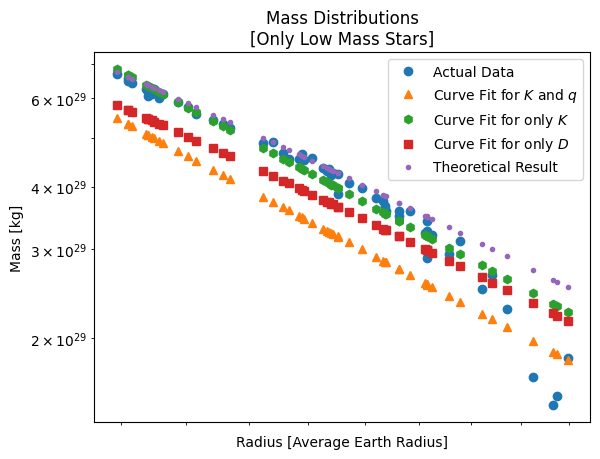
\includegraphics[width=\linewidth]{figures/6_n_ll_m_r_.png}}
%\caption{}
%\label{fig:2_n_ll_rho_m_}
\end{minipage}
\caption{asd}
\label{fig:56}
\end{figure}


\begin{figure}[H]
\begin{minipage}{.5\textwidth}
\centerline{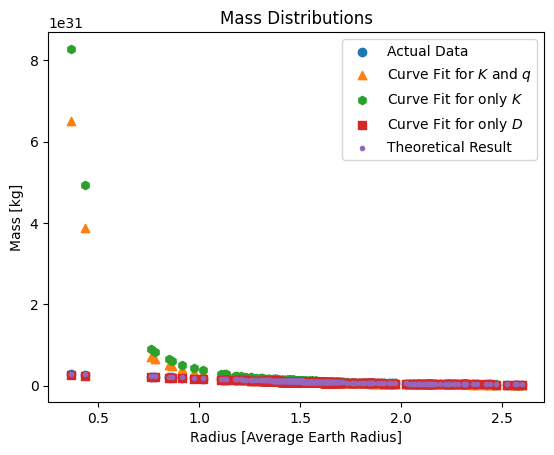
\includegraphics[width=\linewidth]{figures/9_n_s_m_r.png}}
%\caption{}
%\label{fig:1_n_ll_rho_m}
\end{minipage}
\begin{minipage}{.5\textwidth}
\centerline{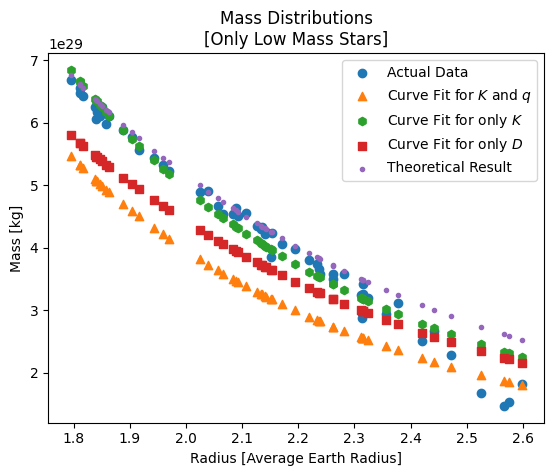
\includegraphics[width=\linewidth]{figures/10_n_s_m_r_.png}}
%\caption{}
%\label{fig:2_n_ll_rho_m_}
\end{minipage}
\caption{asd}
\label{fig:9_10}
\end{figure}
\end{comment}


\subsection{Experimental Results Based on the Relativistic Approach}

\paragraph{} All experiments are conducted based on the preassumed distribution of the central pressure. The range of the assumed central pressure distribution can be observed below:

\begin{equation*}
    p_c = \left\{10^{20}, \dots, 10^{45}\right\} \frac{kg}{m^3} 
\end{equation*}

\paragraph{} In Figure \ref{fig:17_18}, the mass and radius distribution wihch is obtained by the integration of the \eqref{eq:tov} can be observed.
\paragraph{} In Figure \ref{fig:17_18}, the relation between fractional binding energy and radius can be observed. Inspecting the Figure \ref{fig:17_18}, one can infer that as the radius increases, the difference between rest mass and  relative mass decreases. However, in low values of radius, rest mass is relatively higher than the relative mass.

\begin{figure}[H]
\begin{minipage}{.5\textwidth}
\centerline{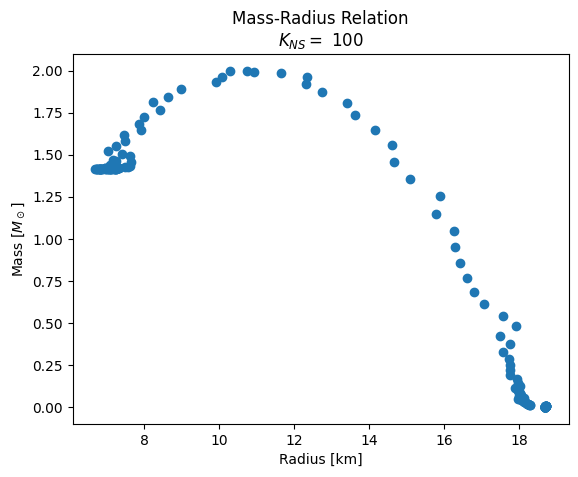
\includegraphics[width=\linewidth]{figures/17_e_s_m_r.png}}
%\caption{}
%\label{fig:1_n_ll_rho_m}
\end{minipage}
\begin{minipage}{.5\textwidth}
\centerline{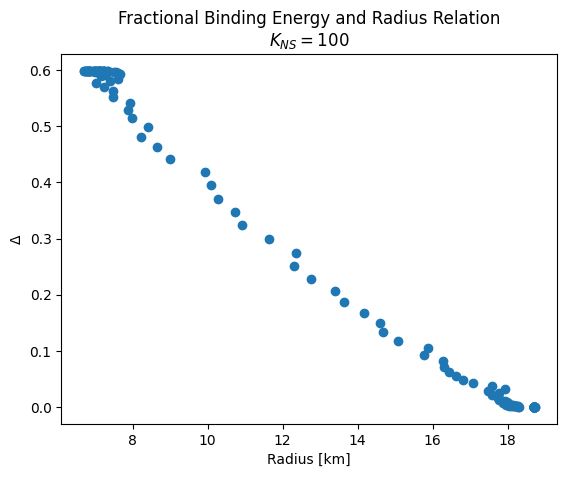
\includegraphics[width=\linewidth]{figures/18_e_s_delta_r.png}}
%\caption{}
%\label{fig:2_n_ll_rho_m_}
\end{minipage}
\caption{The Relation of Radius with Mass and Fractional Binding Energy}
\label{fig:17_18}
\end{figure}

\paragraph{} In Figure \ref{fig:19}, the \textit{log-log} plot that visualizes the relation between mass and central density can be observed. The stability of the point are determined via using the below relation:

\begin{align*}
    \frac{dM}{d_{\rho_c}} > 0 &\Rightarrow Stable \\
    \frac{dM}{d_{\rho_c}} < 0 &\Rightarrow Unstable \\
\end{align*}

\paragraph{} Moreover, in Figure \ref{fig:19}, there is a peak point which actually represents the mass limit that a NS can be enlarged, which also corresponds to the point where the transition from stable region to unstable region starts. This maximal points corresponds to the below numerical value:

\begin{equation*}
    M_{max} \approx 2.0 M_\odot
\end{equation*}

\begin{figure}[H] 
\centering 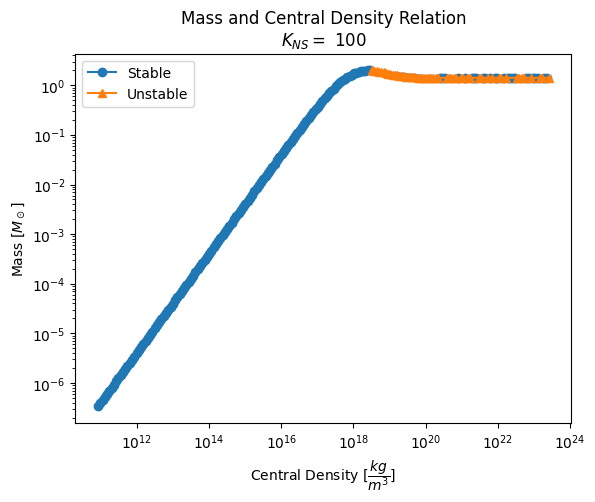
\includegraphics[width=0.7\columnwidth]{figures/19_e_ll_m_rho.png}           
\caption{Mass and Central Density Relation}                
\label{fig:19}
\end{figure}

\paragraph{} As discussed in Section \ref{sec:tov}, the equation of state of the relativistic case is not well-defined. Initially, it is assumed as the polytropic relation with index of $1$. Moreover, as can be observed in Figure \ref{fig:17_18} and Figure \ref{fig:19}, the polytropic constant is chosen as $K_{NS} = 100$. In Figure \ref{fig:20}, the effect of the alteration of the polytropic constant ($K_{NS}$) on the maximum mass that can a neutran star have can be investigated.

\paragraph{} Thanks to the observations done so far, it is known that the heaviest neutron star has the mass of $M = 2.14 M_\odot$, which corresponds to the point that crossed with red lines in Figure \ref{fig:20}. According to the red crosses, it can be concluded that the maximum allowable polytropic constant ($K_{NS}$) reads:

\begin{equation*}
    K_{NS_{max_{allowable}}} \approx 112.5
\end{equation*}
\begin{figure}[H] 
\centering 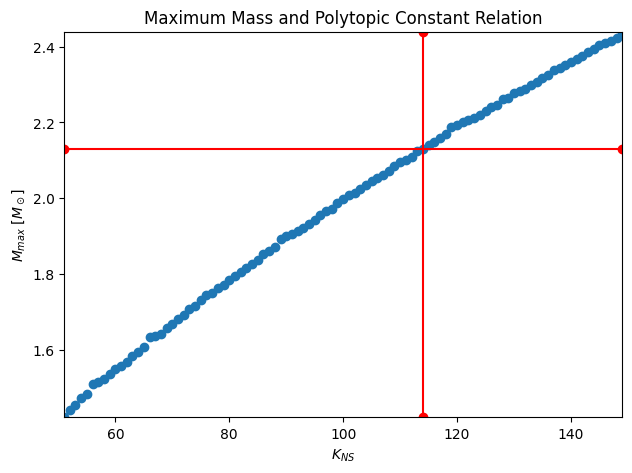
\includegraphics[width=0.7\columnwidth]{figures/20_e_s_m_k.png}           
\caption{Maximum Mass and Polytropic Constant ($K_{NS}$) Relation}                
\label{fig:20}
\end{figure}

\end{document}


              


